\documentclass[journal]{IEEEtran}

% *** CITATION PACKAGES ***
%
%\usepackage{cite}
\usepackage{capt-of}%%To get the caption
\usepackage{gensymb}
\usepackage{graphicx} %package to manage images
\graphicspath{ {./images/} }
\usepackage{wrapfig}

\usepackage[style=ieee]{biblatex}
\DeclareLanguageMapping{english}{english-apa}
\addbibresource{references.bib}
\usepackage[justification=centering]{caption}

\usepackage{setspace}

% *** GRAPHICS RELATED PACKAGES ***
%
\ifCLASSINFOpdf
  % \usepackage[pdftex]{graphicx}
  % declare the path(s) where your graphic files are
  % \graphicspath{{../pdf/}{../jpeg/}}
  % and their extensions so you won't have to specify these with
  % every instance of \includegraphics
  % \DeclareGraphicsExtensions{.pdf,.jpeg,.png}
\else
  % or other class option (dvipsone, dvipdf, if not using dvips). graphicx
  % will default to the driver specified in the system graphics.cfg if no
  % driver is specified.
  % \usepackage[dvips]{graphicx}
  % declare the path(s) where your graphic files are
  % \graphicspath{{../eps/}}
  % and their extensions so you won't have to specify these with
  % every instance of \includegraphics
  % \DeclareGraphicsExtensions{.eps}
\fi
% graphicx was written by David Carlisle and Sebastian Rahtz. It is
% required if you want graphics, photos, etc. graphicx.sty is already
% installed on most LaTeX systems. The latest version and documentation
% can be obtained at: 
% http://www.ctan.org/pkg/graphicx
% Another good source of documentation is "Using Imported Graphics in
% LaTeX2e" by Keith Reckdahl which can be found at:
% http://www.ctan.org/pkg/epslatex
%
% latex, and pdflatex in dvi mode, support graphics in encapsulated
% postscript (.eps) format. pdflatex in pdf mode supports graphics
% in .pdf, .jpeg, .png and .mps (metapost) formats. Users should ensure
% that all non-photo figures use a vector format (.eps, .pdf, .mps) and
% not a bitmapped formats (.jpeg, .png). The IEEE frowns on bitmapped formats
% which can result in "jaggedy"/blurry rendering of lines and letters as
% well as large increases in file sizes.
%
% You can find documentation about the pdfTeX application at:
% http://www.tug.org/applications/pdftex

\begin{document}

\begin{titlepage}
    {\centering
        \vspace*{20em}
        {
        \huge 
        \begin{spacing}{1.5}
            Measuring the Internal Resistance of an \\
            Alkaline and Nickel Metal Hydride Battery

            
            \\
            \\
            \bigskip
            \large
            Circuits Fundamentals Lab 3, (ENGR-UH 2019-LAB)
        \end{spacing}

        }
        
    }
    \vfill
    
    {
    \large
    
    \begin{spacing}{1.5}
    \noindent Barkin Simsek, {\it {bs3528@nyu.edu}} 
    \\
    Nishant Aswani, {\it {nsa325@nyu.edu}}
    \\
    Table Number: \#Workstation 8% <-this % stops a space
    \end{spacing}
    }


\end{titlepage}
\pagenumbering{gobble}
\clearpage\mbox{}
\clearpage
\pagenumbering{arabic}
\setcounter{page}{1}

%\title{Demonstration of a Voltage Divider With A Variable Resistor}

%\author{Barkin Simsek,~\IEEEmembership{bs3528@nyu.edu};
%Nishant Aswani,~\IEEEmembership{nsa325@nyu.edu}
%\\ Table Number: \#}% <-this % stops a space


% The paper headers
\markboth{Simsek, Aswani, Circuits Fundamentals Lab 2019}%
{}

% make the title area
%\maketitle

% As a general rule, do not put math, special symbols or citations
% in the abstract or keywords.
\begin{abstract}
In this experiment a switch controlled LED circuit was built using a $330 \ohm$ resistor, as a visual indicator for the on/off status for a radio receiver to be implemented later. Calculations were carried out to confirm that the resistor value used was appropriate. A simulation was also run for further confirmation. Finally, the circuit was assembled by soldering components onto a prototype board and testing by applying a 9V source.
\end{abstract}


%Percenta of power being consumed at the internal resistence

%What happens to voltage when external load is connected and current %consumption increaased

%Formula derivation
%Application 


\section{Introduction}
\IEEEPARstart{T}\lowercase{he} purpose of this exercise was to measure the internal resistance of a battery using a simple resistor circuit, compare the power absorbed between the internal resistor ($R_{in}$) and the resistor in the circuit ($R_{ex}$), and describe the relationship between the voltage drop and current load across $R_{ex}$. Comparing the power consumption of the internal resistor to that of the load resistor would emphasize the importance of minimizing internal resistance. 

\nonindent In ideal circuit diagrams, it is often assumed that voltage sources provide the voltage they are rated for. Realistically, batteries have an internal resistance, the value for which depends on the type of cell, which has the effect of providing a voltage drop and limiting the current through the circuit. Naturally, a low internal resistance is preferred.

\begingroup
    \medskip
    \centering
    %width=\columnwidth
    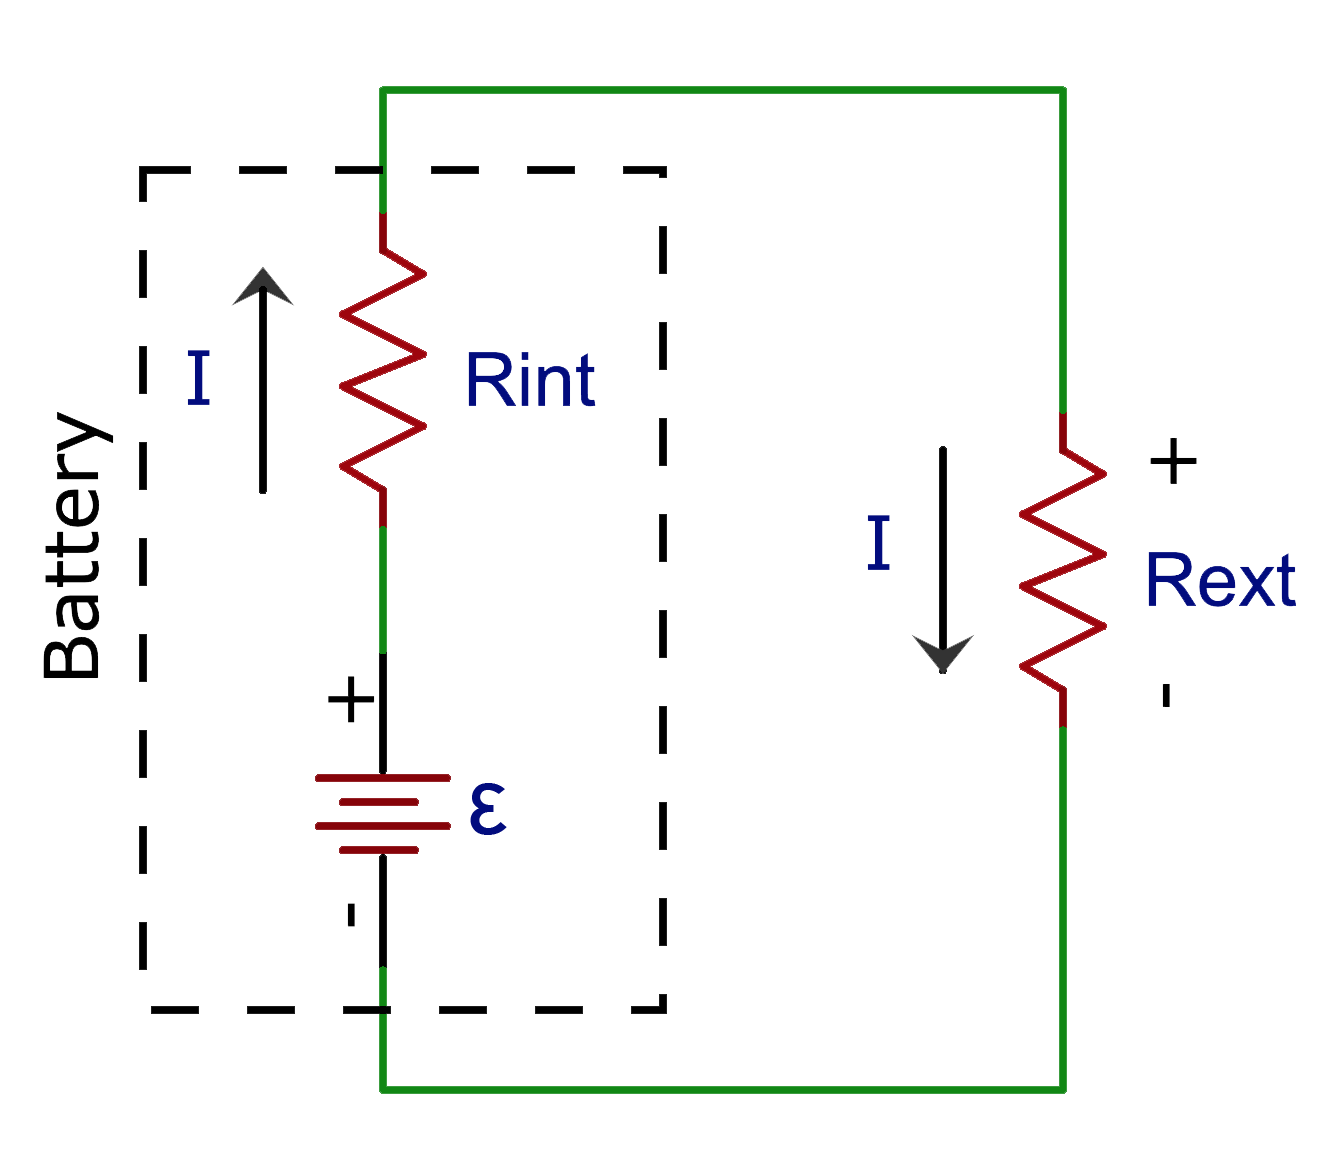
\includegraphics[width=\columnwidth]{images/lab3_1.png}
    \captionof{figure}{A schematic for a modular, \\ switch-controlled led circuit}
    \label{fig:first}
    \medskip
\endgroup

\noindent Figure \ref{fig:first} above simplifies the internal resistance of the battery system (battery, wires, screw terminal, etc.) to a single equivalent resistor. In principal, the internal resistance was determined by measuring the supplied voltage,  the voltage drop across $R_{ex}$, and manipulating Ohm's law to determine the supplied current. 


\smallskip
\section{Circuit Assembly}

\noindent The simple schematic was recreated in CAD as shown in Figure \ref{fig:third}. The simulation illustrates the idea of an internal resistor. Assuming no internal resistance for a battery in an ideal circuit, 

Following the schematic, components were placed onto a breadboard for initial testing (Figure \ref{fig:third}). Later the working circuit was transferred onto a prototyping board and components were soldered. Two screw terminals were placed at either end of the board to allow for battery cables and radio receiver cables to be fed in and out and be replaced if needed. The slide switch was soldered in the middle of the board; the power cable from the battery terminal was soldered to the common pin, while the power cable leading to the radio receiver was soldered to the terminal 2 pin. Thus, the circuit could be opened by sliding the common pin to connect with the terminal 1 pin.\\

\begingroup
    \medskip
    \centering
    %width=\columnwidth
    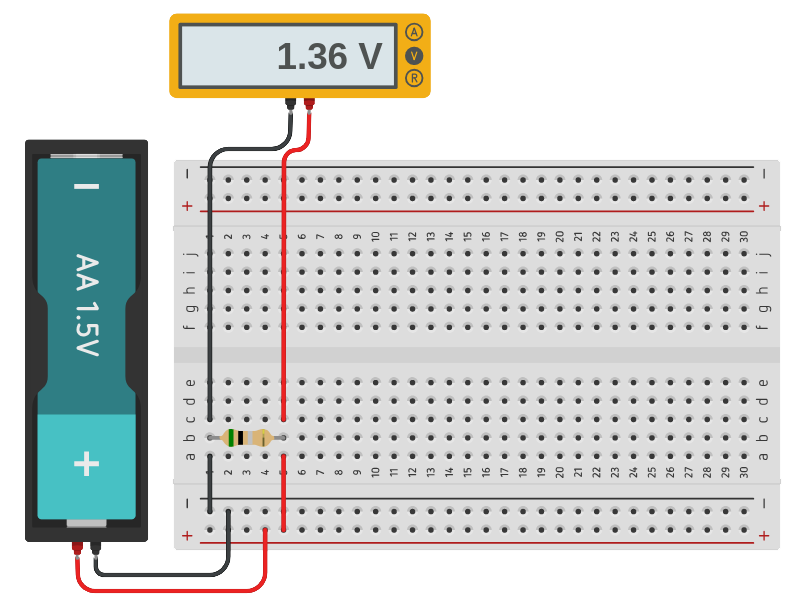
\includegraphics[width=\columnwidth]{images/lab3_2.png}
    \captionof{figure}{CAD layout recreating the switch-controlled circuit.}
    \label{fig:third}
    \medskip
\endgroup

\noindent A cable was directly connected between the negative terminals on both screw terminals.  The anode of the LED was soldered to the negative terminal on the battery terminal for grounding. One leg of the protective resistor was soldered to the terminal 2 pin of the switch, while the other leg of the resistor was soldered to the cathode of the LED, thus completing the circuit (see Figure \ref{fig:second}).

\begingroup
    \medskip
    \centering
    %width=\columnwidth
    \includegraphics[width=\columnwidth]{images/lab2_4.png}
    \captionof{figure}{Switch-controlled circuit to control LED and any attached system.}
    \label{fig:second}
    \medskip
\endgroup


\section{Ohm's Law Calculations}
\noindent The resistance value of the protective resistor is important as it prevents the current from exceeding the maximum specified current for the component. The green LED used was rated for a maximum $30mA$ forward current and 100 $mA$ peak forward current \cite[]{datasheet}. Ohm's law was used to calculate the required resistor values that satisfied the ratings of the LED as shown in Equation \ref{eq:minresistancecalc}.

\begin{equation}
R = \frac{V}{I} = \frac{9V}{30mA} = 300\ohm
\label{eq:minresistancecalc}
\end{equation}

While the calculations imply the use of a $300 \ohm$ resistor for the case of maximum forward current, any resistor value which supplies approximately below $30mA$ (for a reasonably luminescent LED) is appropriate. In this case, a $330 \ohm$ resistor was used as it was the closest resistor value and provided a maximum forward current of $27mA$, which is under the recommended maximum. This decision was confirmed by the simulation (see Figure \ref{fig:fourth}), which shows that using a $330 \ohm$ resistor results in a forward current of $20.9mA$, far less than the recommended $30mA$. The operation of the circuit was also confirmed by soldering the components to a prototype board and supplying $9V$ through the battery terminal resulting in a functional circuit(see Figure \ref{fig:fifth}).

 \begingroup
    \medskip
    \centering
    %width=\columnwidth
    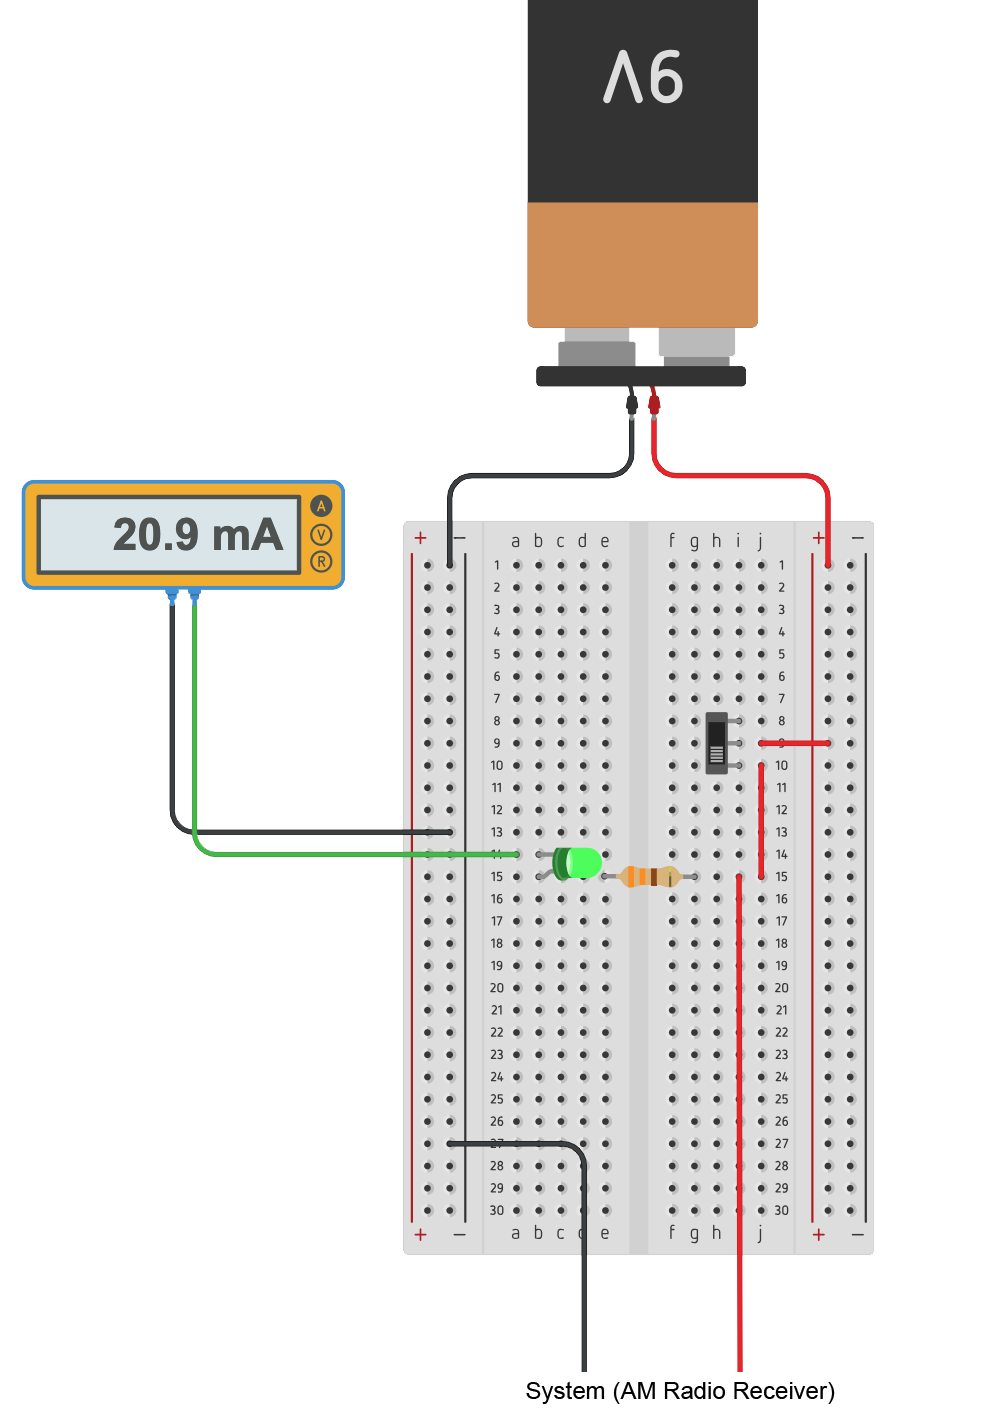
\includegraphics[scale=0.43]{images/lab2_3.png}
    \captionof{figure}{Simulation for $330 \ohm$ resistor in the circuit}
    \label{fig:fourth}
    \medskip
\endgroup

\begingroup
    \medskip
    \centering
    %width=\columnwidth
    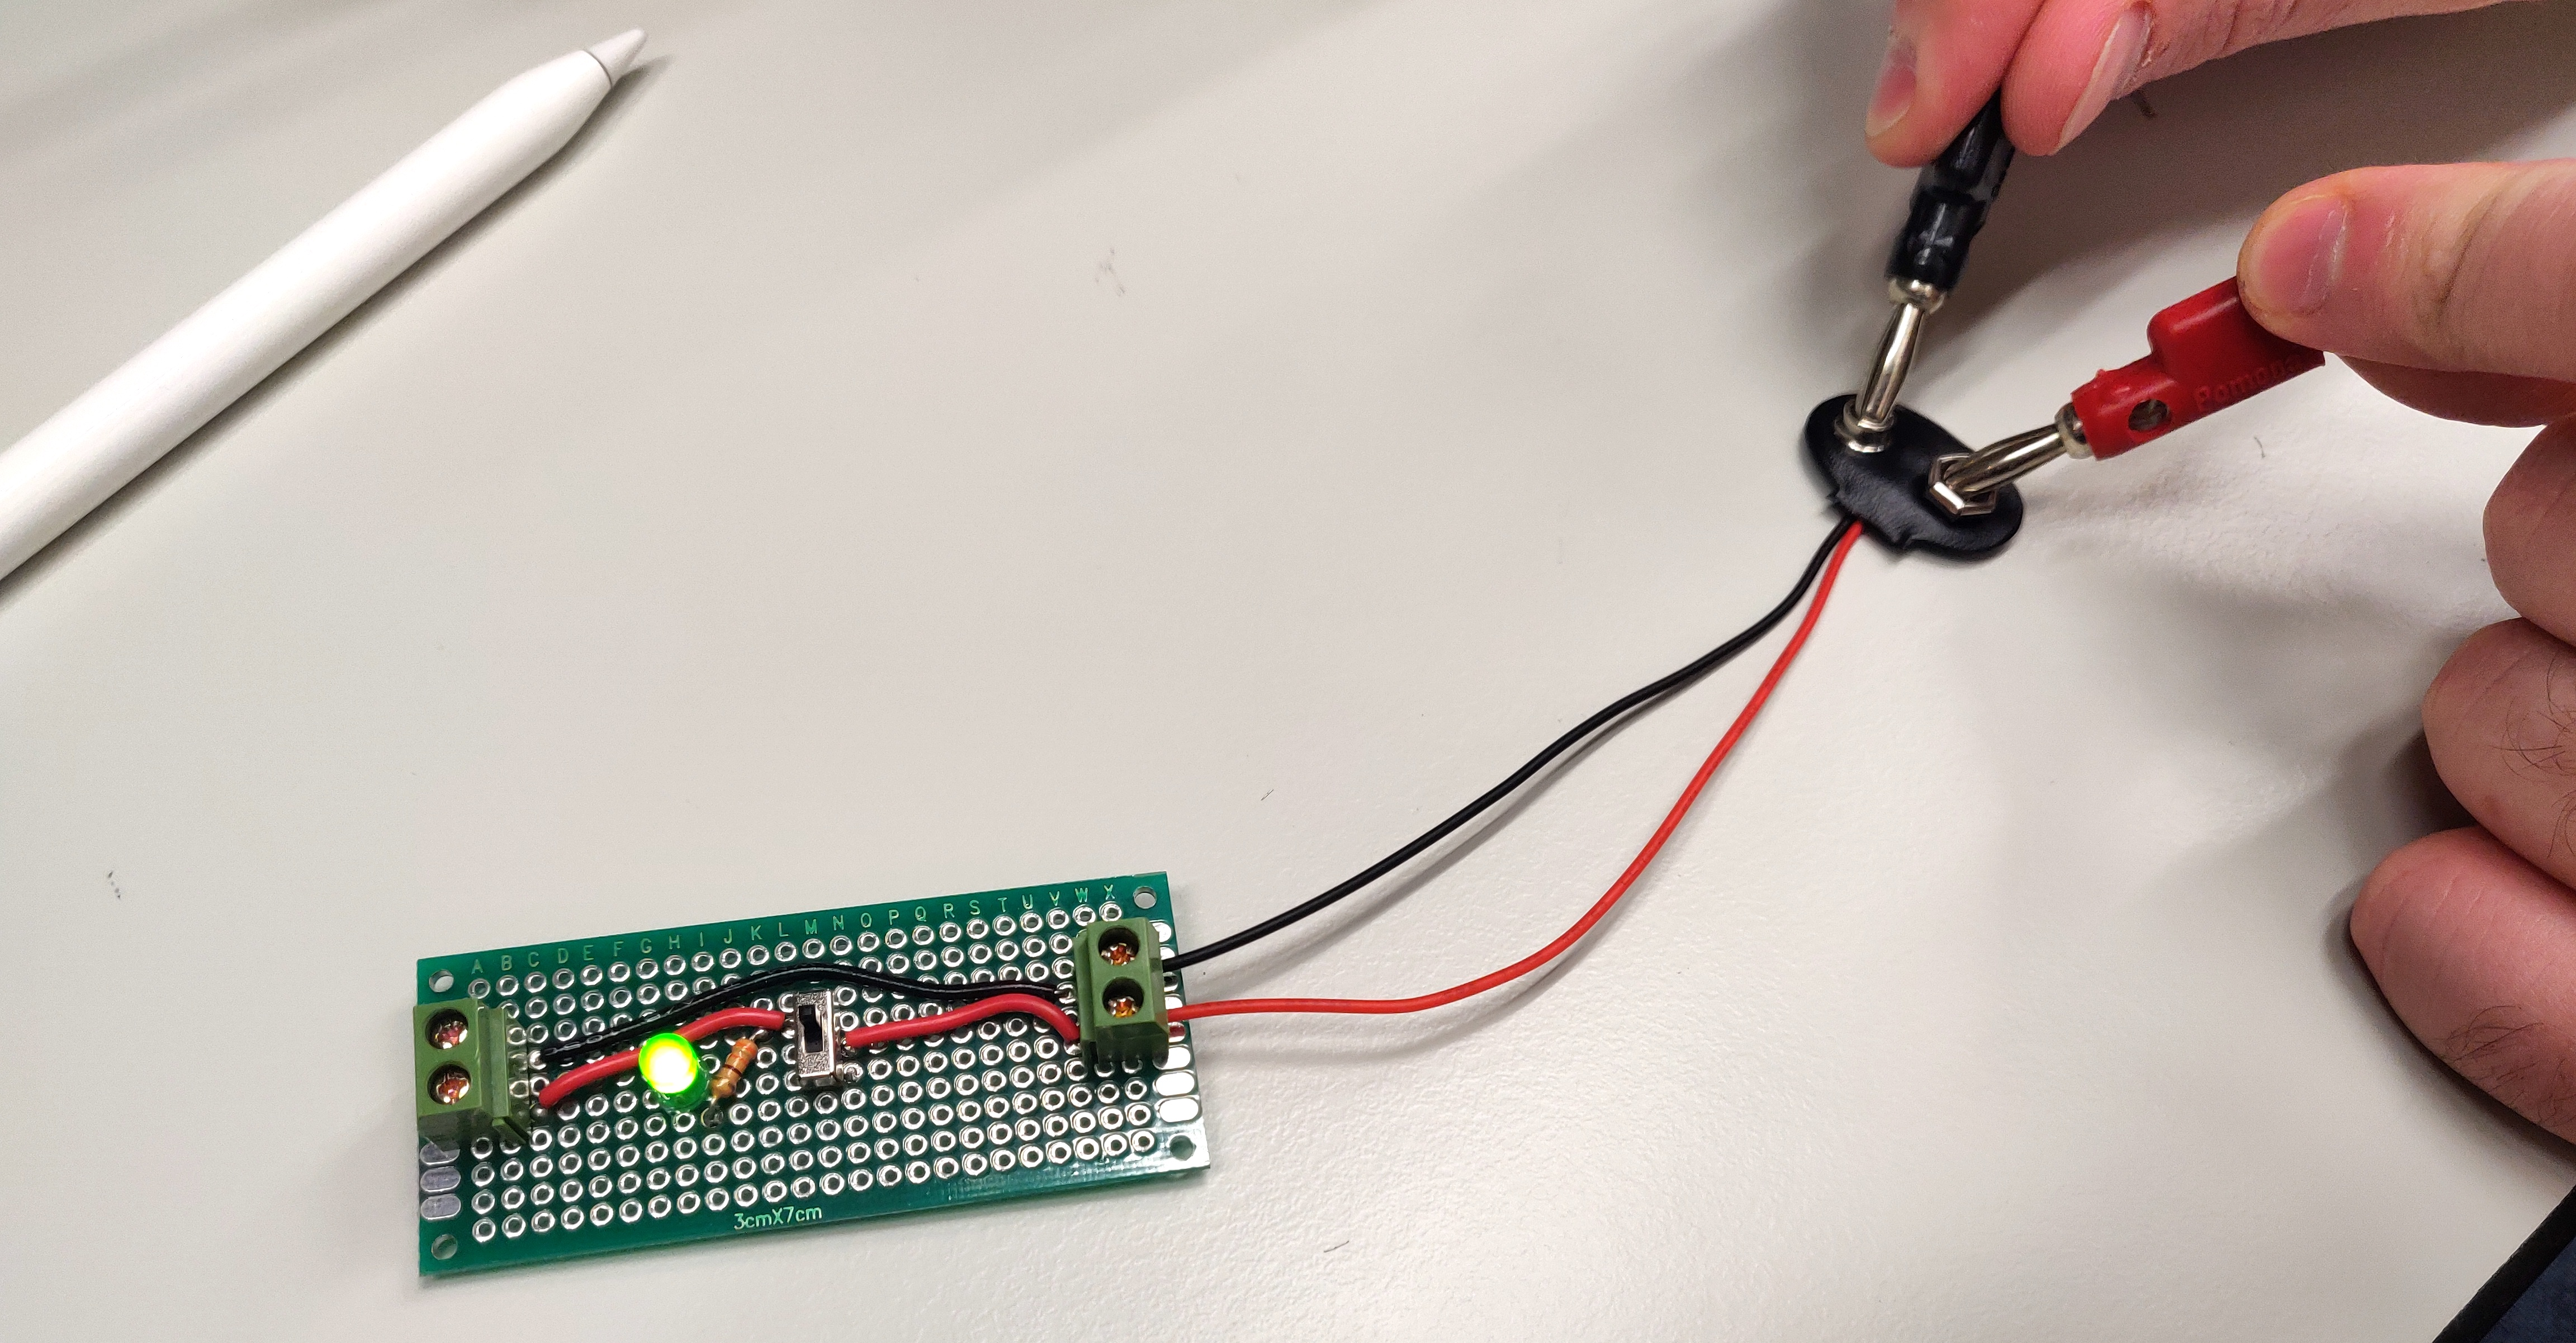
\includegraphics[width =\columnwidth]{images/lab2_5.jpg}
    \captionof{figure}{Final testing of the completed circuit}
    \label{fig:fifth}
    \medskip
\endgroup

\section{Discussion and Conclusion}\\

\noindent A generic power switch for a system (AM radio receiver) was assembled. An LED with a protective resistor was also fitted into the circuit to act as a status indicator. A $300 \ohm$ resistor value was calculated using Ohm's Law assuming peak forward current. The closest resistor value of $330 \ohm$ was used for the circuit, resulting in a forward current of $20.9mA$ and a successful circuit. The lab also acted as an exercise for good soldering practices, such as setting the right temperature and ensuring solder to pad connection, which were critical to the circuit operating when finally assembled. 


%\appendices
%\section{Proof of the First Zonklar Equation}
%Appendix one text goes here.

%\section*{Acknowledgment}

\printbibliography

\end{document}